% The proof chain and its trust boundaries. Build: lualatex pipeline.tex (standalone PDF);
% PNG for README: pdftoppm -png -r 200 -singlefile pipeline.pdf pipeline
\documentclass[tikz,border=4pt]{standalone}
\usepackage{lmodern}
\usetikzlibrary{arrows.meta,positioning,fit,backgrounds}
\definecolor{kern}{HTML}{0072B2}
\definecolor{meas}{HTML}{E69F00}
\definecolor{trust}{HTML}{8C8C8C}
\begin{document}
\sffamily
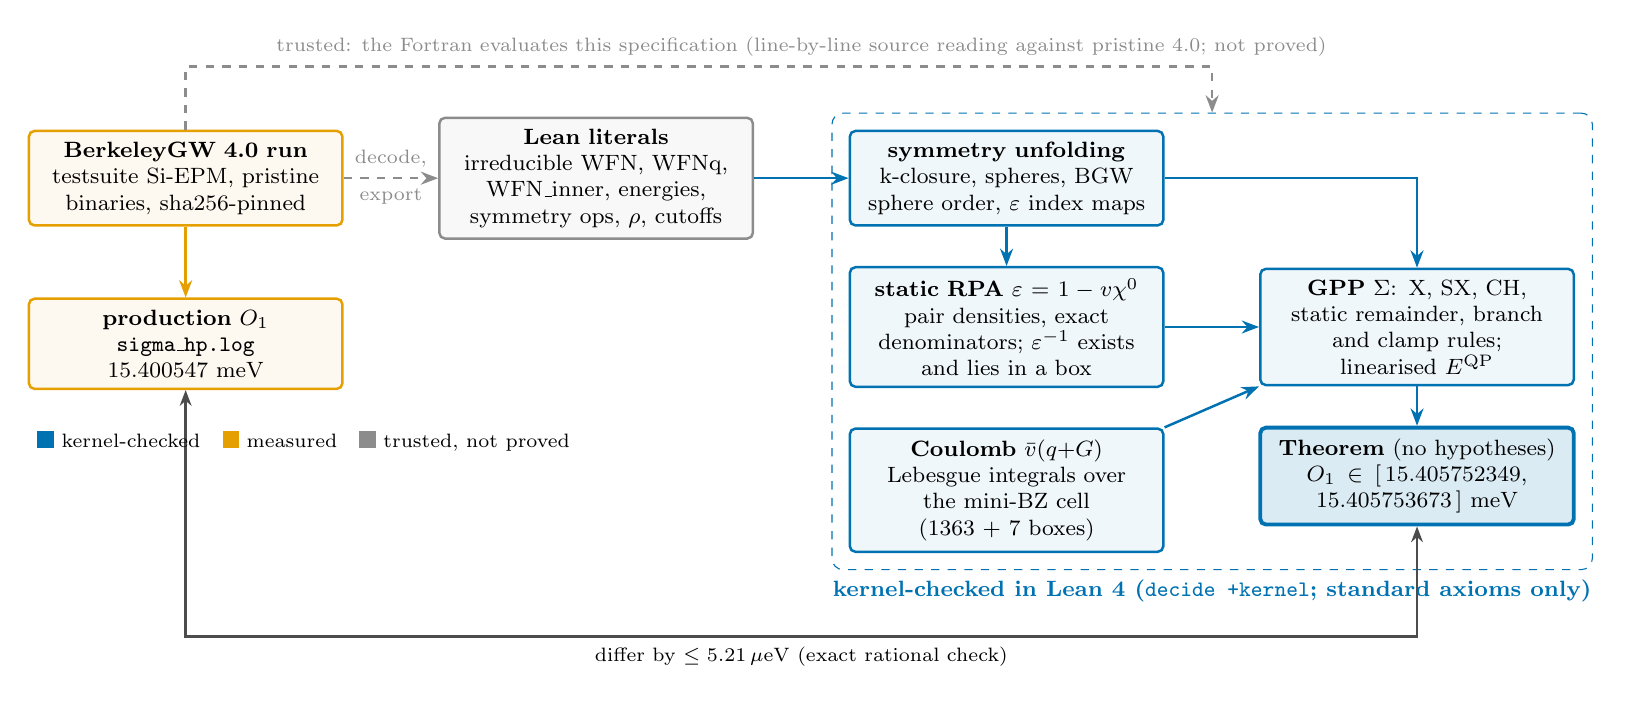
\begin{tikzpicture}[
  node distance=5mm and 7mm,
  box/.style={draw=#1, line width=0.9pt, rounded corners=2pt, align=center, font=\footnotesize,
              inner sep=4pt, text width=37mm, fill=#1!6},
  box/.default=kern,
  arr/.style={-{Stealth[length=2.2mm]}, line width=0.9pt, draw=#1},
  arr/.default=kern,
  lab/.style={font=\scriptsize, align=center, text=#1},
  lab/.default=kern]

% column 1: the run
\node[box=meas] (run) {\textbf{BerkeleyGW 4.0 run}\\ testsuite Si-EPM, pristine\\ binaries, sha256-pinned};
\node[box=meas, below=9mm of run] (prod) {\textbf{production} $O_1$\\ \texttt{sigma\_hp.log}\\ 15.400547 meV};

% column 2: literals
\node[box=trust, right=12mm of run] (lit) {\textbf{Lean literals}\\ irreducible WFN, WFNq,\\ WFN\_inner, energies,\\ symmetry ops, $\rho$, cutoffs};

% column 3: kernel-checked chain
\node[box, right=12mm of lit] (unf) {\textbf{symmetry unfolding}\\ k-closure, spheres, BGW\\ sphere order, $\varepsilon$ index maps};
\node[box, below=of unf] (eps) {\textbf{static RPA} $\varepsilon = 1 - v\chi^0$\\ pair densities, exact\\ denominators; $\varepsilon^{-1}$ exists\\ and lies in a box};
\node[box, below=of eps] (coul) {\textbf{Coulomb} $\bar v(q{+}G)$\\ Lebesgue integrals over\\ the mini-BZ cell\\ (1363 + 7 boxes)};

% column 4: sigma and theorem
\node[box, right=12mm of eps] (sig) {\textbf{GPP} $\Sigma$: X, SX, CH,\\ static remainder, branch\\ and clamp rules;\\ linearised $E^{\rm QP}$};
\node[box, line width=1.4pt, below=of sig, fill=kern!14] (thm) {\textbf{Theorem} (no hypotheses)\\ $O_1 \in [\,15.405752349,$\\ $15.405753673\,]$ meV};

\draw[arr=trust, dashed] (run) -- node[above, lab=trust] {decode,} node[below, lab=trust] {export} (lit);
\draw[arr] (lit) -- (unf);
\draw[arr] (unf) -- (eps);
\draw[arr] (unf.east) -| (sig.north);
\draw[arr] (eps) -- (sig);
\draw[arr] (coul.north east) -- (sig.south west);
\draw[arr] (sig) -- (thm);
\draw[arr=meas] (run) -- (prod);
\draw[{Stealth[length=2mm]}-{Stealth[length=2mm]}, line width=0.9pt, draw=black!70]
  (prod.south) |- node[pos=0.75, below, font=\scriptsize, align=center]
  {differ by $\le 5.21\,\mu$eV (exact rational check)} ([yshift=-14mm]thm.south) -- (thm.south);

\begin{scope}[on background layer]
  \node[draw=kern, dashed, rounded corners=4pt, inner sep=6pt, fit=(unf)(eps)(coul)(sig)(thm),
        label={[font=\footnotesize\bfseries, text=kern]below:kernel-checked in Lean 4 (\texttt{decide +kernel}; standard axioms only)}] (K) {};
\end{scope}

% trusted correspondence
\draw[arr=trust, dashed] (run.north) -- ++(0,8mm) -| node[pos=0.3, above, lab=trust]
  {trusted: the Fortran evaluates this specification (line-by-line source reading against pristine 4.0; not proved)} (K.north);

% legend
\node[anchor=north west, font=\scriptsize, align=left] at ([yshift=-4mm]prod.south west)
  {\textcolor{kern}{\rule{6pt}{6pt}} kernel-checked\quad \textcolor{meas}{\rule{6pt}{6pt}} measured\quad
   \textcolor{trust}{\rule{6pt}{6pt}} trusted, not proved};
\end{tikzpicture}
\end{document}
